%! TEX root = ../main.tex
\documentclass[main]{subfiles}

\begin{document}
\silentchapter{\texorpdfstring
{$\sqrt[n]{\frac{ax+b}{cx+d}}\text{型:}\quad t=\sqrt[n]{\frac{ax+b}{cx+d}}\text{と置換}\rightarrow  t\text{だけの式}$}
{}}

\begin{mondai}{難易度★★★★}{}
    % --- ここから問題パート(上半分) ---
    $$\int ^1_0 \sqrt{\frac{1-x}{1+x}} dx$$
    
    % --- ここで上下を区切る ---
    \tcblower
    
    % --- 解説パートの先頭に「発想」を記述 ---
    \begin{pointbox}
        \begin{center}
        $$\sqrt[n]{\frac{ax+b}{cx+d}}\text{型:}\quad t=\sqrt[n]{\frac{ax+b}{cx+d}}\text{と置換}\rightarrow  t\text{だけの式}$$
        \end{center}
    \end{pointbox}

    % --- ここから解説パート(下半分) ---
    \begin{tcolorbox}
        \begin{align*}
            t=\sqrt{\frac{1-x}{1+x}} \qquad 
            \begin{tabular}{c|ccc}
                $x$ & $0$ & $\rightarrow$ & $1$ \\ \hline
                $t$ & $1$ & $\rightarrow$ & $0$ \\
            \end{tabular} \qquad
            dx=-\frac{4t}{(1+t^2)^2}dt
        \end{align*}
    \end{tcolorbox}
    \begin{align*}
        \int ^1_0 \sqrt{\frac{1-x}{1+x}} dx
            = \int ^0_1 t \left\{ -\frac{4t}{(1+t^2)^2}dt \right\}
            = 4 \int ^1_0 \frac{t^2}{(1+t^2)^2}dt
    \end{align*}
    \begin{tcolorbox}
        \begin{align*}
            t=\tan\theta \qquad 
            \begin{tabular}{c|ccc}
                $t$ & $0$ & $\rightarrow$ & $1$ \\ \hline
                $\theta$ & $0$ & $\rightarrow$ & $\frac{\pi}{4}$ \\
            \end{tabular} \qquad
            dt=\frac{1}{\cos^2\theta}d\theta
        \end{align*}
    \end{tcolorbox}
    \begin{align*}
        %4 \int ^1_0 \frac{t^2}{(1+t^2)^2}dt
            &= 4\int^{\frac{\pi}{4}}_0 \tan^2\theta\cos^4\theta\cdot\frac{d\theta}{\cos^2\theta}
            = 4\int^{\frac{\pi}{4}}_0 \sin^2\theta d\theta \\
            &= 2\int^{\frac{\pi}{4}}_0 \left(1-\cos 2\theta\right) d\theta
            = 2\left[ \theta-\frac{1}{2}\sin 2\theta \right]_0^{\frac{\pi}{4}}
            = 2\left( \frac{\pi}{4}-\frac{1}{2} \right)
            = \frac{\pi}{2}-1 \tag{答}
    \end{align*}

    \begin{figure}[H]
    \centering
    % ★★★ x=5cm, y=5cm でグラフ全体のサイズを大きく見やすく調整 ★★★
    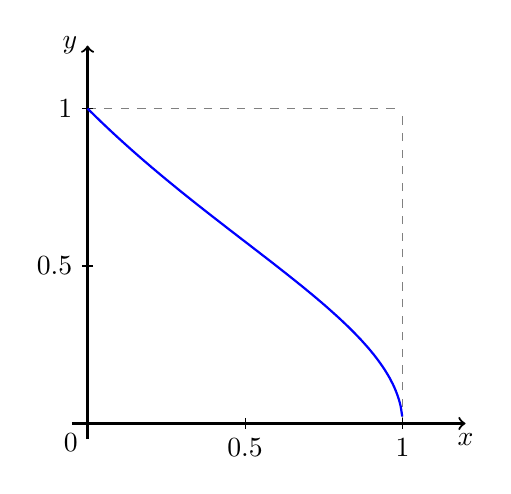
\begin{tikzpicture}[x=4cm, y=4cm]
        % --- 座標軸 ---
        \draw[->, thick] (-0.05,0) -- (1.2,0) node[below] {$x$};
        \draw[->, thick] (0,-0.05) -- (0,1.2) node[left] {$y$};

        % --- グリッド線 ---
        \draw[gray, thin, dashed] (0,1) -- (1,1);
        \draw[gray, thin, dashed] (1,0) -- (1,1);

        % --- 目盛り ---
        \foreach \pos in {0.5, 1} {
            \draw (\pos, 2pt) -- (\pos, -2pt) node[below] {$\pos$}; % x軸
            \draw (2pt, \pos) -- (-2pt, \pos) node[left] {$\pos$};  % y軸
        }
        \node[below left] at (0,0) {$0$};

        % --- グラフのプロット ---
        \draw[
            domain=0:1,
            samples=200, % 急なカーブのためサンプル数を多くする
            smooth,
            variable=\x,
            blue,
            thick
        ] plot ({\x}, {sqrt((1-\x)/(1+\x))});

    \end{tikzpicture}
    \caption{$y=\sqrt{\frac{1-x}{1+x}}$ のグラフ ($0 \le x \le 1$)}
    \label{fig:sqrt_frac_tikz}
    \end{figure}
\end{mondai}

\end{document}